\let\negmedspace\undefined
\let\negthickspace\undefined

\documentclass[journal]{IEEEtran}
\usepackage[a5paper, margin=10mm, onecolumn]{geometry}
%\usepackage{lmodern} % Ensure lmodern is loaded for pdflatex
\usepackage{tfrupee} % Include tfrupee package

\setlength{\headheight}{1cm} % Set the height of the header box
\setlength{\headsep}{0mm}     % Set the distance between the header box and the top of the text

\usepackage{gvv-book}
\usepackage{gvv}
\usepackage{cite}
\usepackage{amsmath,amssymb,amsfonts,amsthm}
\usepackage{algorithmic}
\usepackage{graphicx}
\usepackage{textcomp}
\usepackage{xcolor}
\usepackage{txfonts}
\usepackage{listings}
\usepackage{enumitem}
\usepackage{mathtools}
\usepackage{gensymb}
\usepackage{comment}
\usepackage[breaklinks=true]{hyperref}
\usepackage{tkz-euclide} 
\usepackage{listings}
% \usepackage{gvv}                                        
\def\inputGnumericTable{}                                 
\usepackage[latin1]{inputenc}                                
\usepackage{color}                                            
\usepackage{array}                                            
\usepackage{longtable}                                       
\usepackage{calc}                                             
\usepackage{multirow}                                         
\usepackage{hhline}                                           
\usepackage{ifthen}                                           
\usepackage{lscape}
\begin{document}

\bibliographystyle{IEEEtran}
\vspace{3cm}

\title{4.2.13}
\author{EE25BTECH11010 - Arsh Dhoke}
{\let\newpage\relax\maketitle}

\renewcommand{\thefigure}{\theenumi}
\renewcommand{\thetable}{\theenumi}
\setlength{\intextsep}{10pt}
\numberwithin{equation}{enumi}
\numberwithin{figure}{enumi}
\renewcommand{\thetable}{\theenumi}

\parindent 0px
\textbf{Question}:\\
Find the direction and normal vector for the line 
y = x.

\solution \\

The line can be written as: 
\begin{align}
x - y = 0
\end{align}

This equation can be expressed in terms of matrices\\
Let
\begin{align}
\vec{x} = \myvec{x \\ y}
\end{align}
\begin{align}
\vec{n^T} = \myvec{1 & -1}
\end{align}
\begin{align}
c = 0
\end{align}

The line equation can be written as:
\begin{align}
\vec{n^T}  \vec{x} = c
\end{align}

Where $\vec{n}$ is the normal vector of the given line

The direction vector of the line is:
\begin{align}
    \vec{m} = \myvec{1 \\ 1}
\end{align}

If the director vector is given by
\begin{align}
\vec{m}  = \myvec{1 \\ m}    
\end{align}
then the normal vector can be written as
\begin{align}
\vec{n} = \myvec{-m \\ 1}
\end{align}

We can prove this using
\begin{align}
\vec{n^T}\vec{m} = 0
\end{align}

\begin{align}
\myvec{1 & -1}\myvec{1 \\ 1} = 0
\end{align}

The normal vector of the line is $\vec{n} = \myvec{1 \\ -1}$
The director vector of the line is $\vec{m} = \myvec{1 \\ 1}$\\

\begin{figure}[ht!]
\centering
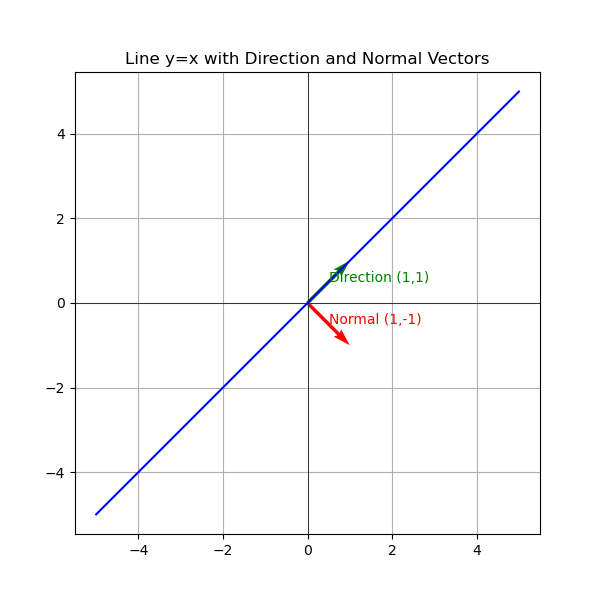
\includegraphics[height=0.6\textheight, keepaspectratio]{figs/q6.png}
\captionof{figure}{Graph}
\end{figure}


\end{document}